% Drawing 147/03-9 -- folder 147, batch 03, archive page 57 (PDF page 58).
% Transcription: les graphes et les courbes du tableau (72), sur trois lignes. Ligne 1 : deux sommets reliés par une arête, marqués « 3 » ($\alpha_0$) et « 2 » (indice surchargé) ; en regard, deux droites qui se coupent, l'une portant $a$, $b$, l'autre $c$, $d$, $e$. Ligne 2 : une boucle fermée sur un sommet marqué « 2 » ($\alpha_0$) ; en regard, une courbe nodale portant $a$ et $b$. Ligne 3 : deux sommets reliés par une arête, le premier ($\alpha_0$, $g_{\alpha_0} = 1$) surmonté d'un chiffre biffé, le second marqué « 2 » ($g_\alpha = 0$) ; en regard, deux branches qui se coupent en un point épais, l'une marquée $g_{\alpha_0} = 1$, l'autre portant $a$ et $b$.
% Kind: three MD-graphs with the curves they stand for. Method 2 (schematic redraw from the facsimile). Status: ok.
% Notes: Three rows, graph on the left, curve on the right. Row 1: an edge between a vertex marked 3 (alpha_0 under it) and a vertex marked 2 (its index, overwritten, is left out, as the transcription cannot read it); two lines crossing at one computed point, the first carrying two ticks a, b, the second three ticks c, d, e. Row 2: a loop closed on a vertex marked 2, (alpha_0) under it; a nodal curve (one self-crossing, a loop below it) with two ticks a and b on the loop. Row 3: an edge between a vertex with (alpha_0) and g_{alpha_0} = 1 under it and a vertex marked 2 with g_alpha = 0 under it; two branches crossing at a heavy point, the left one labelled g_{alpha_0} = 1, the right one carrying two ticks a and b. Left out: the struck figure above the first vertex of row 3 and the struck word above the label g_{alpha_0} = 1 of the curve; the words i.e. and type (0,5), (1,2), (1,2), which the transcription sets in the table. The nodal curve of row 2 is drawn as a smooth curve with the crossing where the page has it. Redrawn 2026-11-12 (issue 128): to check again.
% Coordinates: 1 unit = 1 mm = 1/100 of the crop width (bbox in page fractions: [0.29, 0.585, 0.92, 0.79]).
% Redrawn by Claude (claude-fable-5-2), issue #128, 2026-11-12; not checked by a human; not compiled (no TeX in the session).
% Rights: reproduces part of the work -- behind RENDER_TRANSCRIPTS, never published by itself.
\documentclass[tikz,border=3pt]{standalone}
\usepackage{amsmath,amssymb}
\usetikzlibrary{patterns,arrows.meta}
\tikzset{pencil/.style={black!45}, struck/.style={black!35}, mpt/.style={circle,draw,inner sep=1.3pt}, pt/.style={circle,fill,inner sep=0.9pt}, opt/.style={circle,draw,fill=white,inner sep=1.1pt}}
\begin{document}
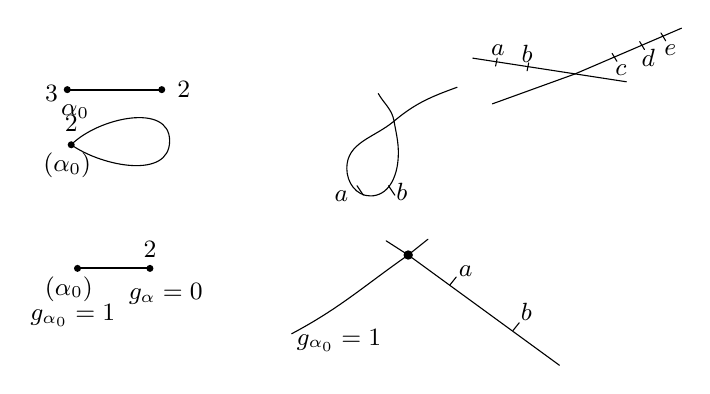
\begin{tikzpicture}[x=1mm,y=1mm,line cap=round,line join=round,font=\scriptsize]
% row 1
\coordinate (P1) at (8,-8);
\coordinate (P2) at (20,-8);
\draw[thick] (P1) -- (P2);
\node[pt] at (P1) {};
\node[pt] at (P2) {};
\node[inner sep=1pt] at (6,-8.5) {\small $3$};
\node[inner sep=1pt] at (9,-10.8) {\small $\alpha_0$};
\node[inner sep=1pt] at (22.8,-8) {\small $2$};
\coordinate (X1) at (72.5,-6);
\draw (59.5,-4) -- (X1) -- (79,-7);
\draw (62,-9.8) -- (X1) -- (86,-0.2);
\draw (62.6,-4) -- (62.4,-5);
\draw (66.6,-4.6) -- (66.4,-5.6);
\draw (77.2,-3.4) -- (77.8,-4.4);
\draw (80.7,-1.9) -- (81.3,-2.9);
\draw (83.4,-0.8) -- (84,-1.8);
\node[inner sep=1pt] at (62.7,-3) {\small $a$};
\node[inner sep=1pt] at (66.4,-3.5) {\small $b$};
\node[inner sep=1pt] at (78.3,-5.5) {\small $c$};
\node[inner sep=1pt] at (81.8,-4) {\small $d$};
\node[inner sep=1pt] at (84.6,-3) {\small $e$};
% row 2
\coordinate (Q) at (8.5,-15);
\draw (Q) to[out=45,in=90] (21,-14.5) to[out=-90,in=-35] (Q);
\node[pt] at (Q) {};
\node[inner sep=1pt] at (8.5,-12.3) {\small $2$};
\node[inner sep=1pt] at (8,-17.6) {\small $(\alpha_0)$};
\coordinate (N) at (49.5,-12);
\draw (57.5,-7.7) to[out=200,in=40] (N) to[out=220,in=90] (43.5,-18) to[out=-90,in=180] (46.5,-21.5) to[out=0,in=-95] (50,-17) to[out=85,in=-80] (N) to[out=100,in=-60] (47.5,-8.5);
\draw (44.8,-20.2) -- (45.6,-21.4);
\draw (48.8,-20.2) -- (49.6,-21.4);
\node[inner sep=1pt] at (42.8,-21.5) {\small $a$};
\node[inner sep=1pt] at (50.5,-21) {\small $b$};
% row 3
\coordinate (R1) at (9.3,-30.7);
\coordinate (R2) at (18.5,-30.7);
\draw[thick] (R1) -- (R2);
\node[pt] at (R1) {};
\node[pt] at (R2) {};
\node[inner sep=1pt] at (18.5,-28.3) {\small $2$};
\node[inner sep=1pt] at (8.2,-33.3) {\small $(\alpha_0)$};
\node[inner sep=1pt] at (8.7,-36.7) {\small $g_{\alpha_0} = 1$};
\node[inner sep=1pt] at (20.5,-34) {\small $g_{\alpha} = 0$};
\coordinate (X3) at (51.3,-29);
\draw (36.5,-39) to[out=28,in=215] (X3) -- (53.8,-27);
\draw (48.5,-27.2) -- (X3) -- (70.5,-43);
\node[pt,inner sep=1.2pt] at (X3) {};
\draw (56.6,-32.8) -- (57.4,-31.8);
\draw (64.6,-38.6) -- (65.4,-37.6);
\node[inner sep=1pt] at (58.6,-31) {\small $a$};
\node[inner sep=1pt] at (66.3,-36.2) {\small $b$};
\node[inner sep=1pt] at (42.5,-39.8) {\small $g_{\alpha_0} = 1$};
\end{tikzpicture}
\end{document}
